\documentclass{article}
\usepackage{geometry}
\usepackage{array}
\usepackage{graphicx}
\usepackage{enumitem}
\usepackage[hidelinks]{hyperref}

\renewcommand{\familydefault}{\sfdefault}
\geometry{a4paper, portrait, margin=2.5cm}
\def\labelitemi{--}
\hyphenchar\font=-1
\graphicspath{{images/}}


\begin{document}

\title{MEng Individual Project Interim Report}
\author{Jake Reynolds}

\maketitle

\tableofcontents

\section{Introduction}
This document contains an Interim Report of my 4th Year MEng project. The project concerns creating a drone with cloud-based AI elements, with conception and execution being done in conjunction with IBM. IBM are providing funding for large purchases, and are acting as a client. They are also providing extended access to their Platform as a Service (Paas) Bluemix. Below is detailed the project specification, background and related research, and details about how the project is being implemented and evaluated.


\section{Project Specification}
\subsection{Motivation}
Whilst there is a growing trend for drone usage in search and rescue operations, this often requires a trained manual operator. With the increasing accuracy and improvements in machine learning techniques, both local and remote AI control of drones is becoming a reality. However, machine learning algorithms often require extensive computational power, and are not suited to be executed locally on a drone. Additionally, any behaviour learned is lost should a drone be destroyed. Cloud services provide a solution to these problems.

\vspace{\baselineskip} \noindent
This project is a proof-of-concept implementation, with the aim that future research and development can be built upon the results; IBM already have in place plans to take this work further after the project's completion. The focus of the project development is for the system to be able to react in a desired manner to certain scenarios that it may encounter in search and rescue environment. These will be used both as a target for development and for evaluation. An initial list of these scenarios can be found at the end of the report. The challenges of cloud systems providing AI are both physical, requiring a reliable internet connection for a mobile drone, and virtual, in requiring many components and services to work together seamlessly.


\subsection{Deliverables}
This project is intended to deliver a system comprising of two main components, the drone and cloud services. The purpose of the drone is to act as a data collector and system actuator, whilst the cloud services combines a variety of data analytical services to inspect the data from the drone and issue appropriate commands.

\subsubsection{Drone}
The `drone' is a self-contained unit consisting of a quadcopter drone frame, being assembled by myself, with an autopilot device attached. This device allows simpler control of the drone, as well as added functionality such as `hover', but despite the name does not provide autonomous flying and navigation. This autopilot can be controlled either via remote, as is typical of drones, or via direct connection through a set of telemetry IO pins. In my `drone', these  will be connected to a Raspberry Pi's GPIO pins, and the Pi is to be carried as a drone payload. The Pi can therefore send signals to the drone autopilot in a similar manner to a remote control, for instance sending the `up' command.

\vspace{\baselineskip} \noindent
The Raspberry Pi will be connected to the internet, initially via a WiFi connection, however this may be changed to a 3G link depending on the requirements of the connection and the level of data transfer. This link provides access to Bluemix, through the HTTP and MQTT protocols. The HTTP connection provides a large data upload link to Bluemix, for example images and audio recordings. This connection is made on a file-by-file basis. The MQTT protocol is different; as it is based on a publisher/subscriber model, it requires a `stay alive' connection to be established initially. Its purpose is to allow movement commands to be pushed to the Pi from Bluemix. Small-size status data will be sent from the Pi to Bluemix, such as GPS coordinates, but it has not yet been established if this will be via the MQTT or HTTP protocols.

\vspace{\baselineskip} \noindent
The Pi will be capable of a variety of data collection methods, however the primary one will be `vision', in the form of a Raspberry PiCam. This is a small, very compact camera connected via a dedicated ribbon cable to the Pi board. It is capable of still images with a resolution of 2592x1944, or video at 1920x1080. In this project I will be using still images, as this allows use of image recognition services which currently don't support video. The secondary data collection method will be audio, collected via an external microphone. Other planned data sources also include temperature and drone location, with both GPS coordinates and altitude.

\subsubsection{Cloud Services}
For reasons explained in further detail within the Background section, the IBM Bluemix platform was chosen to be the primary provider of the cloud services. The `cloud services' deliverable will consist of a system or application which is run in the cloud on a remote server. As stated, this will be run on Bluemix with the application having its own designated domain, currently http://drone-nodes.eu-gb.mybluemix.net/, through which the HTTP REST requests will occur. The server will receive the data uploaded from the drone, and will store it, process it, and return feedback. The central component running on the server will be written in Node.js. The `intelligence', which decides how to reacts to the analysis the services provide, will be written as a Node.js component running on the server.

\vspace{\baselineskip} \noindent
Bluemix services, all provided by IBM, that are expected to be used in the deliverable include:
\begin{itemize}
    \item Cloudant Database. This is a noSQL database built on top of CouchDB. This will be used to store all data, whether raw images from the camera or the results of analysis.
    \item Internet Of Things Foundation. This is a wrapper around an MQTT broker, providing the publisher/subscriber control.
    \item Visual Recognition. Service that takes as input uploaded images and returns a set of labels with associated probability values, which aim to describe what the image depicts.
    \item Speech To Text. A service based on a neural network that analyses input audio and returns transcripts of intelligible speech.
    \item Tone Analyser (experimental). This service analyses a body of text, and aims to return meaningful insights into the tone of message. As explained in the Implementation Plan, this service may not be included in the deliverable.
    \item NodeRED. This service provides a graphical interface for connection of services, based on Node.js. This is used for quickly testing ideas and rapid development, but is perhaps not as suitable for a final deliverable due to issues with customisation.
\end{itemize}


\section{Background}
The use of drones in search and rescue is not only a very active field of research, there are also an increasing number of successful use cases \cite{UAVUseCase}. \emph{Search} can be considered the more important part of search and rescue, as without a person's location known, they cannot be rescued. Unmanned Aerial Vehicles (UAVs) tend to be the most common design of drone used, as they are most suited to helping \emph{search}; from their unique viewpoint, they can gain greater visual information in a much shorter time, especially if more than one drone work in collaboration \cite{UAV}. However, these drones still require a skilled operator, which may either be unachievable or a poor use of limited resources.

\vspace{\baselineskip} \noindent
Although research is being conducted into making drones fully autonomous, as is pointed out by Tomic et al  \cite{Autonomous} UAVs can only support a lightweight payload, which greatly restricts the computing power available. This is especially important for autonomous drones as they rely heavily on machine learning algorithms for functionality such as speech recognition and visual recognition. These are typically dependent on computationally intensive neural networks \cite{Neural}, which currently cannot be deployed on the microprocessors light enough to be used as a UAV payload. Whilst there exist a range of libraries supporting image and speech recognition on mobile devices, these are not suitable for this application due to two major issues; the computational complexity required for higher accuracy, and power consumption. `Offline' techniques do not tend to use neural networks, and are even less likely to use deep neural networks. This is because they require a large amount of mathematical computation when training and using the network; deep neural networks are notoriously hard to optimise \cite{DeepAI}. In theory they can be implemented on small devices such as a Pi, and indeed sometimes are \cite{DeepPi}, but even with the Pi's processor running at maximum image classification can take ~20 seconds. This is much too slow for real-time search and rescue. In addition, power consumption must be considered. In all examples such as the one cited above, the microprocessor has a stable mains power supply. On a drone, there is no such source. The maximum current the Pi can draw is 1A. Given that the Pi takes 300mA when idle, the PiCam module takes another 250mA, a communication module with the ground will require a further 200mA, and peripheral sensors will require another 100mA or so, there is very little room to power the CPU or GPU to implement onboard processing. Whilst computation could be expanded by adding more processors, as is done by Tomic et al \cite{Autonomous}, there comes a point where, given that the lifting capability of the drone is fixed, moving computation off board is the only option.

\vspace{\baselineskip} \noindent
One solution to this problem, which is growing ever more popular, is the use of the `cloud' to carry out large data storage and computationally expensive tasks \cite{Cloud Robotics}. Although not new in concept, given the increase in availability of commercial cloud service providers in recent years the idea of a remote AI is becoming more of a reality. Analysis of cloud computing systems has shown them to have perform well in many desirable areas, such as scalability, portability, and maintainability \cite{Software Architecture}, which are traits that are becoming more important in the digital age. Given that the drone already has a communication link with the ground for control, this requires little expansion in terms of the hardware or power consumption of the drone; the communication module with draw more current as it transmits more frequently, but the device will still consume less power than if it were to implement local computation as described above. An added benefit of cloud services, or conversely a restriction of onboard processing, is being able to use proprietary services, such as the Tone Analysis described later in this report.

\subsection{Cloud Services}
\subsubsection{Providers}
There exist a number of Platform as a Service (PaaS) providers, but three of the most popular are summarised below.
\begin{itemize}
    \item Microsoft Azure - well-established provider, high cost with no free-tier
    \item Google App Engine - offers a free-usage tier, but has more limited machine learning services
    \item IBM Bluemix - more recently released, offers unique `Watson' intelligence.
\end{itemize}
%Suitable approach?
As this project was a collaboration with IBM, Bluemix was the provider chosen. However, there is good reason for this, primarily due to the unique services and functionality which Bluemix provides related to machine learning and data analytics. These have been developed following IBM's success with the intelligent machine Watson, and are likewise named Watson Services \cite{Watson}. The insights provided by these unique services have been experienced by myself in previous work with Bluemix \cite{EdgeOfSpace}, and verified by recent research to test Bluemix's capabilities \cite{Sentiment}. Especially relevant services that Bluemix provides, which are not available from alternative PaaS providers, are the Visual Recognition and Tone Analysis services.

\subsubsection{Architectural Advantages}
Bluemix, as well as many other PaaS systems, utilises the microservices architecture. This is in contrast to the `traditional' monolithic approach, when all of a system's functionality and processing is conducted centrally on a single device. All components are interdependent, and should one fail, the whole system fails. Microservices is an alternative architecture, where each component provides a service separately. Components can and should be deployed independently, ideally physically as well as virtually, meaning that should one fail, others are unaffected \cite{Microservices}. Having each component independent allows greater flexibility, providing a high level of scalability and maintainability. Should an update or change of a component be needed, it can be executed without affecting the rest of the system's functionality, resulting in a more reliable and available system.



\section{Implementation Plan}
After the project began, three major milestones were set out, with one allocated for each term. A brief summary is given here, with more details and expansions below. These are quite neatly divided into setup, implementation, and optimisation.

\vspace{\baselineskip} \noindent
\begin{tabular}{p{5cm} p{10cm}}
    \textbf{To Be Accomplished By} & \textbf{Milestone} \\
    Christmas (25/12/2015) & Initialise Bluemix and the Pi, and establish communication. Source drone. \\
    Easter    (22/04/2016) & Have the system infrastructure in place. This includes all services, a central server linking them, and connection with the drone. \\
    Summer    (10/06/2016) & Optimise the system, in terms of latency, throughput and accuracy. Evaluate, improve, expand. \\
\end{tabular}

\vspace{\baselineskip} \noindent
The Christmas milestone was met, and the Easter milestone is currently expected to be completed on time as well. Further details of the work done, and planned future work, are lain out below.

\subsection{Christmas Milestone}
The hardware choices were made early, to maximise the time available for development, and to allow for delays in the procurement of hardware. Different drone designs were considered, such as ground-based versus flying, but an airborne drone was decided upon once clearing had been given for more substantial funding; flying drones offer more advantages in terms of being able to gain greater views, and have potentially more freedom of movement to access physical locations that other designs could not. This is of obvious use for the situations described in the motivation section.

\vspace{\baselineskip} \noindent
A quadcopter drone was decided on, as it gives high manoeuvrability, a good level of lift to accommodate the weight of the payload, whilst still being affordable \cite{UAVDevelopment}. Given the ever increasing numbers of quadcopter drones, there is also a better level of support available. The Unmanned Tech S500 model was chosen as it met all the requirements described above whilst being a suitable cost for IBM to purchase. The suitability of this model for the task was verified by discussion within a specialist drone forum. Along with the physical aspect of the drone, such as frame and motors, an autopilot is needed to be able to control the drone's movement. A Pixhack was chosen as it allows commands to be sent to it directly over provided telemetry pins \cite{Mavlink}.

\vspace{\baselineskip} \noindent
A microcontroller was needed on the drone, to be able to transmit and receive data to and from the cloud, and to connect with the autopilot as described above. A Raspberry Pi was chosen as it offers many benefits, including low cost, relatively high-processing power, and a large amount of support and documentation. It also allows scripting in Python, which is the language of choice for the `drone' section of this project. Python allows very fast scripting and easy integration of both web services and GPIO pin control, and the speed benefits of alternative languages such as C are not required. The Pi also provides a dedicated connection for a camera, the PiCam, which can be used for image capture.

\vspace{\baselineskip} \noindent
After initial speed in choosing the drone, there was a slow down due to IBM's lack of speed in providing a Bluemix account and issues with purchasing the drone. Eventually, I was required to ask my supervisor to sign up to IBM's Academic Initiative to obtain a Bluemix account, which was done near the start of December. After obtaining this account, I was able to rapidly establish a connection between the Pi and Bluemix using cURL, and the NodeRED service. After difficulties in trying to get the Image Recognition service to work correctly with images uploaded from the Pi, the way the central component is developed was changed, and is currently based on Node.js and an express server. This allows for a far higher level of control and customisation, but results in slower development.

\vspace{\baselineskip} \noindent
Despite providing IBM with details of the expensive hardware that was needed on the 6/11/2015, I have yet to receive any parts. This is primarily due to supply issues with the vendor; shortly after choosing the drone model it went out of stock from the only UK vendor. IBM Procurement have been diligently following this up, and I am regularly updated. Some components have already arrived, and all the hardware should be with me in the near future.

\subsection{Easter Milestone}
The target by the end of Easter is to have, in essence, the entire system functioning correctly. This means that if the system is given a suitable input, a scenario trigger occurs (as described in Scenarios), and the respective action is taken. The work this involves, with deadlines, can be summarised as follows:

\vspace{\baselineskip} \noindent
Drone
\begin{itemize}
    \item Receive and assemble drone (T + 14 days, with T being the day the drone is received)
    \item Connect Raspberry Pi to autopilot and check functionality (T + 14)
    \item Write scripts to carry out data collection and forwarding to Bluemix (T + 21)
    \item Write scripts to execute commands returned from Bluemix (T + 21)
\end{itemize}

\vspace{\baselineskip} \noindent
Cloud Services
\begin{itemize}
    \item Create all relevant Bluemix services (Complete)
    \item Connect to Bluemix services with central express server (Complete)
    \item Create relevant paths from REST endpoints to the Bluemix services (Complete)
    \item Handle the analysis returned from the appropriate services (11/03/2016)
        \begin{itemize}
            \item Image Recognition (Complete for subset of labels)
            \item Speech Recognition (Complete for generic non-empty transcript)
            \item Tone Analysis/Natural Language Classifiers
            \item Implement internal services, such as temperature warnings and air purity measurements
        \end{itemize}
    \item Be able to execute any and all appropriate actions (25/03/2016)
        \begin{itemize}
            \item Send movement commands to the drone (Complete), and implement them
            \item Raise flags within system, send to Android app (Complete, see Expansions)
            \item Log analysis in database (Complete)
        \end{itemize}
\end{itemize}

\vspace{\baselineskip} \noindent
The deadlines for Drone targets above are somewhat flexible, given the delay with the procurement of the drone as described above. When the drone arrives, it should be assembled as soon as possible to ensure that all necessary hardware has been obtained and that the vital link between the Pi and the drone works as expected. Ample time has been allowed for assembly as it is a process that should not be rushed, as an error could be costly both in terms of time and money.

\vspace{\baselineskip} \noindent
During the first few weeks of Spring term, I have taken advantage of the fact that there is less going on in terms of other requirements, and have invested time into the project. This has resulted in me achieving many of the targets for Cloud Services already. However, the last item is the most involved and complex, so will require the most work.

\subsection{Summer Milestone}
By the start of this stage, the entire system should be functioning correctly end to end, with the majority of the functionality in place. This should give plenty of time for project optimisation and evaluation. Should extra time be available, there are a range of potential future expansions that could be considered as an additional extension.

\subsubsection{Optimisation}
The optimisation of the system will include testing the system against a set of metrics, identifying bottlenecks and see where improvements can be made. Examples of metrics to test include:
\begin{itemize}
    \item End to end latency - from data capture to command execution
    \item End to end throughput - how many images per minute, is constant audio recording achievable?
    \item Service response - if the image recognition takes x seconds, can it process another request within this time?
    \item Communication bandwidth - how much data can be transmitted between the drone and Bluemix? Can the data be compressed or reduced somehow? 3G vs WiFi?
\end{itemize}
After identifying issues, appropriate action will be taken. Examples of actions include considering alternative data compression methods from JPEG/WAV and limiting server requests to an appropriate level to ensure optimum throughput. Should bandwidth be a major issue, reducing the quantity of data sent could be considered, as well as simply compressing as mentioned above. This could mean doing initial primitive image or sound analysis onboard the Pi, and should any results be found then the data could be sent to Bluemix for more detailed processing. This is certainly feasible for sound analysis, as low-powered speech recognition tool boxes exist, albeit with low accuracy. However, it is less likely to be possible for the image recognition, as this is more computationally difficult.

\vspace{\baselineskip} \noindent
Each of these metrics are important in their own right. Latency is of course an important issue in a search and rescue operation, where time is of the essence. For instance, a delay of 30 seconds for image recognition is unacceptable, as it will slow down the entire search operation. Similarly, throughput is an obviously important metric; unless all terrain can be inspected, all sounds analysed, the effectiveness of the search operation is greatly reduced. The system should aim for real-time analysis of all input stimuli. Service response, whilst not being under my control, is an important aspect to understand, both as a baseline for the rest of the system, and for potential workarounds for instance in service request concurrency. Communication is a characteristic of the system that underpins both latency and throughput, and indeed the reliability of the whole system, so must be well understood and optimised.

\subsubsection{Evaluation}
The evaluation of the system will be primarily based around scenarios which represent situations the drone may encounter in its proposed use. More details of this process can be found in the Evaluation Plan.


\subsection{Services Being Used}
This section details the Bluemix services being used to date, including a brief description and thoughts on initial use.


\begin{figure}[h]
\caption{Architectural design of the system}
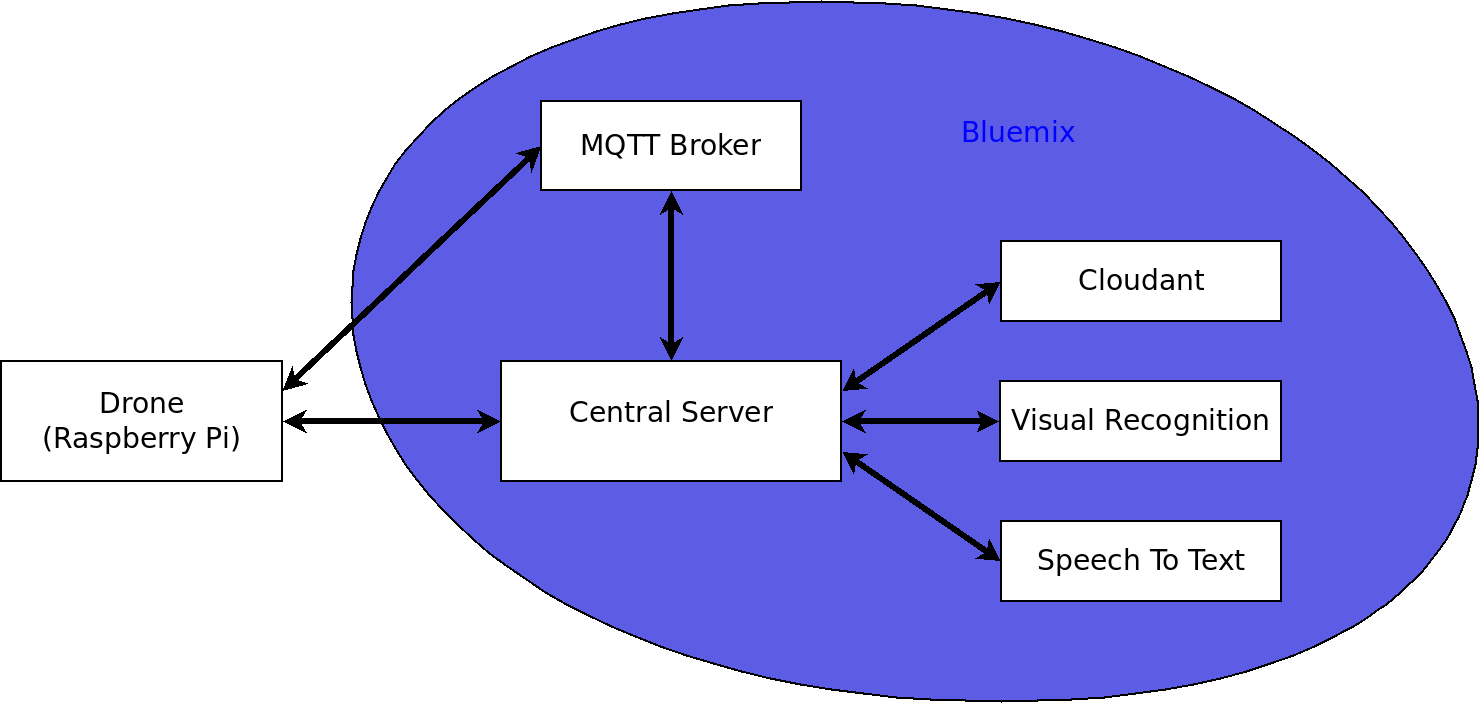
\includegraphics[width=\textwidth]{Architecture}
\end{figure}



\subsubsection{Bluemix Overview}
Bluemix is operated through a browser interface, allowing graphically the simple creation and monitoring of services. Each service has its own dashboard for more detailed configuration and monitoring, for instance allowing database management. Although initially it appears clear and easy to use, it can sometimes feel unreliable and difficult to know how to do exactly what is wanted. Unreliability issues arise when trying to do implement any major changes to the structure of an application, by adding or removing a service, or by restarting the application. This results in the application `restaging', a rather slow process which can occasionally fail without information as to why. Support is also somewhat lacking, likely due to the recency of Bluemix's release. Whilst there is documentation, it can be hard to find specific details, and there is little help on external forums. Many of the issues I have experienced with Bluemix are known and understood, as shown by am IBM-commissioned usability report \cite{Bluemix}. Nevertheless, the power of the interface is impressive, with the ability to start a template application that uses multiple services within minutes.

\subsubsection{Central Server}
A component is required to link all of the other services together, and to coordinate communication between them. This `central server' layer between external devices and the Bluemix services not only provides this functionality, it allows custom processing of the analysis, and a layer of abstraction. Devices therefore only have to connect to one endpoint for all analysis. Initially, this was developed using NodeRED, a browser based graphical editor based on Node.js. It allows different services to be connected very simply, and allows very rapid development. However, it is in some ways too high-level. Finding the cause of errors is very tricky, which is an issue when learning about Bluemix and its services. For instance, if an image was uploaded to the Visual Recognition service, but the format was wrong, an unidentifiable and uncaught error is thrown causing the application to reboot, which means the browser editor becomes unavailable for 5 minutes. Although later I discovered these issues can be somewhat mitigated by developing locally, development of the central component is currently being done directly in Node.js.

\vspace{\baselineskip} \noindent
Development in Node.js required a steep learning curve, as I have not used JavaScript before. It can be very powerful, but has many features I am not used to. Currently this component consists of a passive server, which on initialisation creates connections to all of the services detailed below, and describes a REST API for the drone to use. It then awaits the use of this API, where it receives files, forwards these to the relevant services, and awaits analysis results. Once these have arrived, the results and interpreted and relevant commands are generated, often resulting in commands sent to the MQTT service and information logged in the database.

\subsubsection{Database}
To store all the data that is captured, along with analysis results, a database is needed. Bluemix supports two main types, an SQL and a noSQL (Cloudant). The Cloudant database was chosen the system has to store a lot of images. Not only did the SQL implementation have a data limit of 50MB on the Free Tier version of Bluemix, but it is less suited for storing files such as JPEGs. Alternative free databases were explored, such as freesqldatabase\cite{FreeSQL}, however these all had similar size limitations, much less than the 20GB Cloudant option. A database created and hosted by myself would have been possible, allowing me to have virtually unlimited space, however it was both highly inefficient time-wise and would have had a comparatively low data bandwidth, being run on a standard desktop PC over domestic internet.

\vspace{\baselineskip} \noindent
The Cloudant database is initially very easy to use, given that it requires no definition like an SQL database. Data input is simple from the express server, using a provided wrapper around the Cloudant's REST API. However, querying is very unlike SQL and was difficult to grasp the concepts of.

\subsubsection{MQTT Communication}
A publisher/subscriber model is ideal for this kind of infrastructure, with a number of connected devices giving constant status updates and receiving commands \cite{Microservices}. It is extremely scalable, requiring no changes should the number of drones using the system be increased in the future. IBM provide the Internet of Things Foundation (IoTF), an adaptation of the MQTT model that provides extra functionality. For instance, it adds a layer of security by only allowing pre-registered devices to connect. It also provides a distinction between events, such as device status, and commands, which can be useful for design clarity. I have previous experience with the IoTF, and know it to be a useful and powerful implementation of MQTT, with an existing library for Python.

\subsubsection{Visual Recognition}
Bluemix provides a Visual Recognition based on a convolutional neural network that can process images and return a set of labels with associated probabilities. However, initial tests resulted in limited success. Note, these were preliminary and minimal tests. Uploaded sample images returned a set containing very variable labels, sometimes contradictory, with very similar probabilities. The complete set of labels is also somewhat limited, and often omits desirable labels for this project. For example, the label `Fireworks' and `Wild\_Fire' exist but simply `Fire' doesn't. The service also has a fairly high latency, requiring a few seconds before the set of labels is returned. This is latency of the service, not of the data transfer. Although this is unavoidable due to the nature of the service, it is possible that multiple queries can be run in parallel, resulting in a better throughput than the latency would indicate.

\vspace{\baselineskip} \noindent
Fortunately, the service allows training of the network, and definition of new labels. In the Summer optimisation phase, I hope to be able to train the service with datasets of images, creating more suitable and applicable labels. In addition, this project is proof-of-concept, and in the future it is likely that the accuracy and label set of this service will improve; unless an `opt-out' header is set, all image data given to the service can be used to improve its accuracy. Neural networks of this scale take a long time and a large dataset to train sufficiently, so the current accuracy levels are inevitable due to how recently the service was released.

\subsubsection{Speech To Text}
Speech To Text is a well understood and researched machine learning problem, as highlighted by IBM's own research into the area \cite{Science}. IBM's Speech To Text service, similar to the Visual Recognition, is based on neural networks. Initial tests resulted in fairly high-levels of accuracy, as to be expected from a modern speech recognition service.

\subsubsection{Tone Analyser}
One of the more experimental services that Bluemix provides in the Tone Analysis, which is based on Natural Language Classifiers. It takes a block of text as input, and outputs sentiment analysis by evaluating the tone of individual words within the text. Initial tests were disappointing, with simple sentences such as ``I am angry'' or ``I need help'' resulting in little usable response. Looking in more depth at provided examples, it seems that the service may require a larger input than a short sentence to generate meaningful analysis. Unfortunately, for the application of this project in search and rescue, it is unlikely that extensive lengths of text will be generated from the speech of people the drone encounters. The service may therefore be unsuitable. However, after relating this to an IBM Watson developer, it was suggested to investigate the Natural Language Classifier tool as a substitute. This will be attempted in the near future.

\section{Fallbacks and Expansions}
\subsection{Fallbacks}
The nature of a microservices architecture, combined with an agile approach to the project, mean that expansions and fallbacks for the `cloud' deliverable present themselves focused on the presence of certain components. For example, visual and speech recognition are the two primary methods of analysis, so this functionality and related services should be make to work correctly before attempting to develop the more experimental and less necessary parts such as tone analysis. Indeed, this is how the project has proceeded so far. Should difficulties be met later, then a safe fallback position is ensured in the form of an already working system, albeit with less functionality.

\vspace{\baselineskip} \noindent
In terms of the `drone' deliverable, there is the potential for unexpected issues arising from the assembly of the drone frame and associated control. However, although it is a fairly complex operation, it is not essential to the functioning of the system, and a suitable fallback would be to omit the physical side, and simply prove that the Pi is sending the correct commands to the designated GPIO pins. This is, however, undesirable and would somewhat limit the ability to test the system with real data.

\subsection{Expansion}
A viable and interesting expansion is that of an Android app. This would provide both inputs and outputs to the system, and would be a crucial link between an operator and the system during the development stages of UAV use in search and rescue. It would connect to both the MQTT service and use the central REST API. The app can be used to control movement of the drone, via the MQTT service, with two D pads, similar to a remote. The REST API can be used to regularly load the latest image received from the drone, essentially creating an image stream of the drone's view to help the user pilot the drone. In theory this should allow remote control of the drone from anywhere, as long as both the controller and the drone have a reliable internet connection. Finally, the MQTT service can be used to receive details pushed from the central service regarding the results of analysis. Without this, the only way to view the results of analysis are from viewing the server log, which is less than ideal during testing when controlling the drone.

\vspace{\baselineskip} \noindent
During the Christmas break, my Bluemix account was briefly suspended as it came to the end of the trial period. Whilst waiting for it to be unlocked, I began work on this expansion, and aim to complete it concurrently with the main project. Although it is non-essential, and will be the part of the project left incomplete if needed, I believe it complements the other two deliverables. Starting with the IBM Starter App \cite{IBMMessaging}, so far the connection to the MQTT service has been implemented, with the associated D pad controllers. This has been tested, with the IoT service dashboard correctly showing movement commands from the app. The image stream has also been implemented and tested, with the central server having an appropriate endpoint to retrieve the latest image from the database. The final functionality described above will be implemented soon, but should not require too much time or effort. Although much of the behind-the-scenes work for the app has been implemented, much work is still needed on the interface. Development has been done so far on a smartphone, but a larger screen such as a tablet is required to take full advantage of the image stream and drone control simultaneously. This hardware has yet to be sourced.

\vspace{\baselineskip} \noindent
Given the current rate of development, and providing no major issues are encountered with the sourcing or physical construction of the drone, the project is expected to be completed as specified on time.

\subsection{Potential Future Expansions}
Following the completion of this project, there are a range of potential expansions that may be explored in the future. If time allows, a couple of these expansions may be considered in this project. These include:
\begin{itemize}
    \item Self-navigation and route planning of the drone around a provided map
    \item Generation of a map from the drone's route and sensor measurements
    \item Better way of presenting data, such as plotting flagged events on a map, or providing an interface to access logged data
    \item Expansion of the system to accommodate multiple drones. Given the design and structure of the system, this should require minimal work
    \item Searching for a known or provided face within a crowd, using Facial Recognition
\end{itemize}


\section{Evaluation Plan}
The evaluation of the system will revolve around testing the drone's response to given scenarios which represent situations the drone may encounter in its proposed use. An initial test set of these are detailed below in the Scenarios section.

\vspace{\baselineskip} \noindent
Once the system is ready for evaluation, the scenario will be presented to the system, either in-situ eg by viewing a person, or with simulated inputs in the case of more extreme triggers such as fire or explosion. If the system acts as expected, the input will satisfy the trigger condition(s) and the corresponding action will be executed correctly. These scenarios attempt to represent a wide range of potential input stimuli, and will test all methods of system data capture and output. Some are simpler than others, with a single trigger and an simple output action of adding the event to a log. Others are more involved, testing many aspects of the system at once.

These situations test all aspects of the system. Initially, the data capture techniques register the stimuli. The communication systems are tested as the data is sent to the Bluemix server. The server processing is tested as it forwards data to each service, and processes the returned analysis. Whilst I cannot alter the results obtained from the IBM services, these can be tested as a baseline for understanding the response of the system as a whole. The `AI' of the central server is then evaluated as it generates an appropriate command or response, and forwards it to the drone where the visual actuation such as movement can be inspected.


\subsection{Scenarios}
Below is a list of scenarios that the drone might encounter during its application in the field. ``Raise flag" can cover a range of actual actions, for instance informing the expansion app to log a message, or to generate an alert and change the background colour.  \\


\vspace{\baselineskip}
{
\hyphenchar\font=-1
\centering
\begin{tabular}{| >{\centering\arraybackslash}m{2cm} | >{\centering\arraybackslash}m{2.5cm} | p{5cm} | p{5cm} |}
    \hline
    Name & Description & Trigger & Action \\ \hline
    Fire & \vspace{\baselineskip} A fire is present &
    \begin{itemize}[topsep=0pt, leftmargin=0cm,itemindent=.5cm,labelwidth=\itemindent,labelsep=0cm,align=left]
        \item Image Recognition returning a related label, such as “Wild\_Fire”
        \item Temperature sensor recording an abnormal temperature, eg >40C
    \end{itemize} &
    \begin{itemize} [topsep=0pt, leftmargin=0cm,itemindent=.5cm,labelwidth=\itemindent,labelsep=0cm,align=left]
        \item Send avoidance movement commands to the drone, such as to increase altitude
        \item Raise flag, log occurrence and location of drone
    \end{itemize} \\ \hline

    Person & \vspace{\baselineskip} A person is present &
    \begin{itemize} [topsep=0pt, leftmargin=0cm,itemindent=.5cm,labelwidth=\itemindent,labelsep=0cm,align=left]
        \item Image Recognition returning a related label, such as `person', `adult', `child'
        \item Speech to Text returning a viable result
    \end{itemize} &
    \begin{itemize} [topsep=0pt, leftmargin=0cm,itemindent=.5cm,labelwidth=\itemindent,labelsep=0cm,align=left]
        \item Halt movement of drone to allow operator to act suitably
        \item Raise flag, log occurrence and location of drone
    \end{itemize} \\ \hline

    Building & \vspace{\baselineskip} A building is detected &
    \begin{itemize} [topsep=0pt, leftmargin=0cm,itemindent=.5cm,labelwidth=\itemindent,labelsep=0cm,align=left]
        \item Image Recognition returning a related label, such as “Rural\_Building”
    \end{itemize} &
    \begin{itemize} [topsep=0pt, leftmargin=0cm,itemindent=.5cm,labelwidth=\itemindent,labelsep=0cm,align=left]
        \item Log occurrence, attempt to log location of building
    \end{itemize} \\ \hline

    Explosion & \vspace{\baselineskip} An explosion has occurred &
    \begin{itemize} [topsep=0pt, leftmargin=0cm,itemindent=.5cm,labelwidth=\itemindent,labelsep=0cm,align=left]
        \item Image Recognition returning a related label, such as “Explosion”
        \item A sudden large noise on the drone microphone
    \end{itemize} &
    \begin{itemize} [topsep=0pt, leftmargin=0cm,itemindent=.5cm,labelwidth=\itemindent,labelsep=0cm,align=left]
        \item Halt movement until operator can act suitably ie move drone away, or the Fire scenario occurs
        \item Raise flag, log occurrence
    \end{itemize} \\ \hline

    Smoke & \vspace{\baselineskip} Smoke is present &
    \begin{itemize} [topsep=0pt, leftmargin=0cm,itemindent=.5cm,labelwidth=\itemindent,labelsep=0cm,align=left]
        \item Image Recognition returning a related label, such as “Smoke”
    \end{itemize} &
    \begin{itemize} [topsep=0pt, leftmargin=0cm,itemindent=.5cm,labelwidth=\itemindent,labelsep=0cm,align=left]
        \item No avoidance needed, indeed smoke may be a useful marker to investigate
        \item Raise flag, log occurrence
    \end{itemize} \\ \hline

    Person in Distress & \vspace{\baselineskip} A person is in need of assistance &
    \begin{itemize} [topsep=0pt, leftmargin=0cm,itemindent=.5cm,labelwidth=\itemindent,labelsep=0cm,align=left]
        \item Speech Recognition transcript containing key words, such as ``help'' or ``danger''
        \item Tone Analysis returns analysis indicating stress, anger or a request
    \end{itemize} &
    \begin{itemize} [topsep=0pt, leftmargin=0cm,itemindent=.5cm,labelwidth=\itemindent,labelsep=0cm,align=left]
        \item Further to action of scenario ``Person'', the request should be forwarded to a relevant display device
        \item Raise flag, log occurrence
    \end{itemize} \\ \hline


\end{tabular}
}

\pagebreak
\section{Appendices}
\subsection{Drone Hardware Components}
\begin{itemize}
    \item Raspberry Pi, with a 32GB MicroSD card loaded with Raspbian OS
    \item Raspberry PiCam, a small camera connected via ribbon cable to the Pi
    \item S500 Quadcopter Frame
    \item Pixhack Autopilot
    \item 4x Unmanned Tech 2217Q 880kV Brushless Motors
    \item 4x Gemfly 12" Rotors
    \item Unmanned Tech Quattro 4x 30A Electronic Speed Control
    \item Assorted sensors, which come bundled with the Pixhack
\end{itemize}

\subsubsection{To Be Purchased}
\begin{itemize}
    \item Radio receiver/transmitter for drone control
    \item Battery for drone
    \item Additional sensors, such as temperature
\end{itemize}


\subsection{Code Documentation}
\begin{itemize}
    \item Bluemix Documentation \url{https://www.ng.bluemix.net/docs/}
    \item Watson Services REST API \url{https://watson-api-explorer.mybluemix.net/}
    \item Watson Services Node.js implementation \url{https://github.com/watson-developer-cloud}
    \item IBM Android Starter App \url{https://github.com/ibm-messaging/iot-starter-for-android}
\end{itemize}

\subsection{Further Reading}
A list of references and papers that haven't been used for citation within this report, but were used either for general background reading or may be used in future documentation.
\begin{itemize}
    \item D. Uckelmann, M. Harrison, F. Michahelles, \textit{``An Architectural Approach Towards the Future Internet of Things''}
    \item A. Ulmestig, \textit{``Applications of Cloud Based Cognitive Computing''}
    \item H. Derhamy, J Eliasson, J. Delsing, \textit{``A survey of Commercial Frameworks for the Internet of Things''}
    \item M. Hussan, W. Zhao, J. Yang, \textit{``Provisioning Web Services From Resource Constrained Mobile Devices''}
\end{itemize}

\bibliographystyle{abbrv}
\begin{thebibliography}{20}
    \bibitem{UAVUseCase}
    Account of UAV use in a natural disaster. Published 2th March, 2015. Accessed 21st January, 2016. \\
    \url{https://www.microdrones.com/en/news/detail/uav-surveillance-in-earthquake-stricken-cangyuan/}
    \bibitem{UAV}
    S. Waharte, N. Trigoni, \textit{``Coordinated Search With Swarm of UAVs''}, InSensor, Mesh and Ad Hoc Communications and Networks Workshops, 2009. SECON Workshops' 09. 6th Annual IEEE Communications Society Conference on 2009 Jun 22 (pp. 1-3). IEEE.
    \bibitem{Autonomous}
    T. Tomic et al, \textit{``Towards a Fully Autonomous UAV''}, Robotics and Automation Magazine, IEEE 19.3 (2012): 46-56.
    \bibitem{Neural}
    H. Soltau, G. Saon, \textit{``Joint Training of Convolutional and Non-Convolutional Neural Networks''}, to Proc. ICASSP (2014).
    \bibitem{DeepAI}
    Y. Bengio, \textit{"Learning Deep Architectures for AI"}, Foundations and Trends in Machine Learning 2:1-127
    \bibitem{DeepPi}
    S. Hickson, \textit{"Classifying everything using your RPi Camera: Deep Learning with the Pi"} \\
    \url{http://stevenhickson.blogspot.co.uk/2015/03/classifying-everything-using-your-rpi.html}
    \bibitem{Cloud Robotics}
    D. Lorencik, P.Sincak, \textit{``Cloud Robotics: Current trends and possible use as a service''}, Applied Machine Intelligence and Informatics (SAMI), 2013 IEEE 11th International Symposium on. IEEE, 2013.
    \bibitem{Software Architecture}
    A. Sharma, M. Kumar, S. Agarwal, \textit{``A Complete Survey on Software Architectural Styles and Patterns''}, Procedia Computer Science 70 (2015): 16-28.
    \bibitem{Watson}
    Upbin, Bruce (November 14, 2013). \textit{``IBM Opens Up Its Watson Cognitive Computer For Developers Everywhere''}. Forbes. Accessed 20th January, 2016. \\
    \url{http://www.forbes.com/sites/bruceupbin/2013/11/14/ibm-opens-up-watson-as-a-web-service/}
    \bibitem{EdgeOfSpace}
    J. Reynolds et al, \textit{``Edge Of Space Project Report''}, Imperial College London, 28th June 2015.
    \bibitem{Sentiment}
    N. Shankar Das, M. Usmani, S. Jain, \textit{``Implementation and Performance Evaluation of Sentiment Analysis Web Application in Cloud Computing''}, Computing, Communication and Automation (ICCCA), 2015 International Conference on. IEEE, 2015.
    \bibitem{Microservices}
    D. Namiot, M. Sneps-Sneppe, \textit{``On Micro-services Architecture''}, International Journal of Open Information Technologies ISSN: 2307-8162 vol. 2, no. 9, 2014
    \bibitem{UAVDevelopment}
    Y. Naidoo, R. Stopforth, G. Bright, \textit{``Development of an UAV for Search and Rescue Applications''}, AFRICON, 2011. IEEE, 2011.
    \bibitem{Mavlink}
    Tutorial for connecting autopilot device to a microcontroller, \\
    \url{http://dev.ardupilot.com/wiki/raspberry-pi-via-mavlink/}
    \bibitem{Bluemix}
    A. Siagain, L. Kumar, L. Huang, M. Nguyen, \textit{``IBM Bluemix: Usability Evaluation''}
    \bibitem{FreeSQL}
    FreeSQLDatabase, a website offering an online SQL database service. \\
    \url{http://www.freesqldatabase.com/}
    \bibitem{Science}
    `Science behind the service', detailing IBM's research into speech recognition. Accessed 21st January, 2016. \\
    \url{https://www.ibm.com/smarterplanet/us/en/ibmwatson/developercloud/doc/speech-to-text/science.shtml}
    \bibitem{IBMMessaging}
    IBM Start For Android App. Accessed 21st January, 2016. \\
    \url{https://github.com/ibm-messaging/iot-starter-for-android}

\end{thebibliography}




\end{document}
